\section{The End of the Golden Age}

\begin{quotex}
Two birds, inseparably united companions, dwell in the same tree; the one eats of the fruit of the tree, while the other looks on without eating.

\flright{\textit{Mundaka Upanishad iii.1}}

\end{quotex}

\begin{wrapfigure}{rt}{.3\textwidth}
 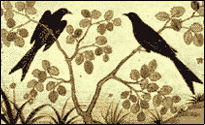
\includegraphics[scale=.5]{a20110112TheEndoftheGoldenAge-img001.png} 
\end{wrapfigure}

This quote from the Upanishads, which appear at the end of the Vedic period, demonstrates the vague beginnings of the dualistic consciousness, the indicator of the transition from one age to the next. At that time, there was still an awareness of the true Self and its connection to the empirical ego, or ``analog I". The latter is active in the natural world, eating its fruits, while the former is the unmoved mover, still in communion with supernature. The rupture, which would later result in the forgetting of the true Self, was not total.

\paragraph{Two Cracks in the Egg}
The empirical I is born as a result of friction: yes and no, good and evil, self and other. This involves judgment and planning, creating a space for reflective thought between contemplation and action. What could intrude in that way into the harmony of the Primordial State? Fabre d'Olivet postulates two events, one internal, the other external.

\subparagraph{Man and Woman}
\begin{quotex}
To enjoy before possessing is the instinct of man; to possess before enjoying is the instinct of woman. 

\flright{\textsc{Fabre d'Olivet}}

\end{quotex}
In this difference in the fundamental attitudes between the sexes, reflection begins. The man pursues, the woman flees; he offers her his gifts, she accepts; he enjoys, she possesses. This primal relationship is the foundation of society. The pact is that the ``stronger was pledged to protect the weaker and the weaker to remain attached to the stronger." This pact extended to the children, which otherwise would have been impossible, and thence to the extended family.

Taken to unnatural direction, the woman became more interested in ``possession", and began to see her husband as a means rather than an end, and developed a sort of matriarchy within the household. This weakened the pact, so man, in reaction, reverted to the instinct of pleasure. His eyes turned to other, younger, women, leading, of course, to conflict. Within the kinship group, this was manageable. But when freed from such constraints through contacts with outsiders, the instinct for possession would lead a woman to the seemingly more prosperous, and man to the more enjoyable, regardless of the consequences.

\subparagraph{Great War}
\begin{quotex}
When it has been necessary to write laws has been when laws were no longer unanimous.

\flright{\textsc{Fabre d'Olivet}}

\end{quotex}
Based on a story from the \emph{Mahabharata}, Fabre d'Olivet then postulated a great war between the Hyperboreans and the Meridional peoples. The various Hyperborean tribes were forced to unite in order to fend off the invasion. But in the General Will there was no clear idea about how to proceed. Out of the confusion, one strong man arose and declared he had a plan. This was the Herman (Gherman), the chief of men. Whereas previously, roles and castes had arisen naturally and organically, the Herman had to explicitly divide the gathered men into three categories.

\begin{enumerate}
\item All the venerable men not able to endure the fatigues of war 
\item All the young and robust men, which constituted the army 
\item The weak and the old who were still active and would provide for the material needs 
\end{enumerate}
This is the beginning of a more formal caste system: the spiritual caste, the warrior caste, and finally the skilled and servile worker castes. This division would outlive its necessity leading to social inequalities, or a fortiori the awareness of social inequalities, with the concomitant possibility of resentment.



\flrightit{Posted on 2011-01-12 by Cologero }

\begin{center}* * *\end{center}

\begin{footnotesize}\begin{sffamily}



\texttt{KarlH on 2011-01-13 at 00:40 said: }

How and why did the Third Sex emerge? Is it due to this same degeneration of will? Does the Third Sex exist (and how)? Does it have a substance of its own in this emerging duality or does it come after it?

I'm referring to both basic Hijra (gender-male but adopting a female way of life) and those who live as both men and women. Is it a taking-of-turns between the two polarities? Is it the consequence of realizing both the masculine and feminine ideals? Theoretically, could one born into this condition be inherently closer to the Absolute in terms of the formlessness that precedes divison?


\hfill

\texttt{kadambari on 2011-01-17 at 01:12 said: }

``I'm referring to both basic Hijra (gender-male but adopting a female way of life) and those who live as both men and women. Is it a taking-of-turns between the two polarities?"

In our tradition these people are considered oddities and are not important. Just as homosexuals are considered not important. People are too intelligent to think they deserve any attention as long as they do not upset the traditional order. Homosexuality is prevalent amongst Muslims in Kashmir, and we see it mostly as a Muslim phenomenon, most of the Muslim rulers of India were bi-sexual, we see this coming from Muslim influence. We cannot relate to such phenomena. I think Hindus were smart to realize that certain types of people cannot be coerced from being what they are, the best thing is to ignore them and not encourage them. That is why unlike Muslims they do not seek to punish such people, but ignore them and do not let them disrupt the traditional order. Ironically those that seek to punish these people such as Muslims have the highest incidence of that which they seek to punish. Just as in Kashmir they are known for being prosmicuous and having the highest divorce rates. Wearing a burka does not indicate anything or any purity as people think.


\end{sffamily}\end{footnotesize}
